%
%
% Tables should be cell-based and may not contain:
% - spacing/line breaks within cells to alter layout or alignment
% - do not nest tabular environments (no tabular environments within tabular environments)
% - no graphics or colored text (cell background color/shading OK)
% See http://journals.plos.org/plosone/s/tables for table guidelines.
%
% For tables that exceed the width of the text column, use the adjustwidth environment as illustrated in the example table in text below.
%
% % % % % % % % % % % % % % % % % % % % % % % %
%
% -- EQUATIONS, MATH SYMBOLS, SUBSCRIPTS, AND SUPERSCRIPTS
%
% IMPORTANT
% Below are a few tips to help format your equations and other special characters according to our specifications. For more tips to help reduce the possibility of formatting errors during conversion, please see our LaTeX guidelines at http://journals.plos.org/plosone/s/latex
%
% For inline equations, please be sure to include all portions of an equation in the math environment.  For example, x$^2$ is incorrect; this should be formatted as $x^2$ (or $\mathrm{x}^2$ if the romanized font is desired).
%
% Do not include text that is not math in the math environment. For example, CO2 should be written as CO\textsubscript{2} instead of CO$_2$.
%
% Please add line breaks to long display equations when possible in order to fit size of the column. 
%
% For inline equations, please do not include punctuation (commas, etc) within the math environment unless this is part of the equation.
%
% When adding superscript or subscripts outside of brackets/braces, please group using {}.  For example, change "[U(D,E,\gamma)]^2" to "{[U(D,E,\gamma)]}^2". 
%
% Do not use \cal for caligraphic font.  Instead, use \mathcal{}
%

\documentclass[11pt,letterpaper]{article}
%\usepackage{CormorantGaramond}
\usepackage{amsmath,amssymb}
%\usepackage{svg}[inkscape=false]
\usepackage{framed}
\usepackage{mdframed}
% Use adjustwidth environment to exceed column width (see example table in text)
\usepackage{changepage}



% textcomp package and marvosym package for additional characters
\usepackage{textcomp,marvosym}
%\usepackage[style=numeric,sorting=none,backend=biber]{biblatex}
%\addbibresource{export.bib}  % Ensure correct .bib filename
\usepackage[T1]{fontenc}
\usepackage{lmodern}

% cite package, to clean up citations in the main text. Do not remove.
%\usepackage{cite}

% Use nameref to cite supporting information files (see Supporting Information section for more info)

\usepackage{svg}
\usepackage{svg-extract}
\usepackage[hidelinks]{hyperref}
\usepackage{nameref}%
\usepackage{float}
%\usepackage{natbib} %
%\usepackage[square,numbers,sort&compress]{natbib}
%\bibliographystyle{plos2015} 
\usepackage[section]{placeins}

%\usepackage{biblatex}

%\bibliographystyle{vancouver}
\usepackage[backend=biber,style=vancouver]{biblatex}
\addbibresource{export.bib} %Import the bibliography file
% line numbers
%\usepackage[right]{lineno}
\usepackage{adjustbox}
% ligatures disabled
\usepackage[nopatch=eqnum]{microtype}
\DisableLigatures[f]{encoding = *, family = * }

% color can be used to apply background shading to table cells only
 %\usepackage[table]{xcolor}

% array package and thick rules for tables
\usepackage{array}

% create "+" rule type for thick vertical lines
\newcolumntype{+}{!{\vrule width 2pt}}

% create \thickcline for thick horizontal lines of variable length
\newlength\savedwidth
\newcommand\thickcline[1]{%
  \noalign{\global\savedwidth\arrayrulewidth\global\arrayrulewidth 2pt}%
  \cline{#1}%
  \noalign{\vskip\arrayrulewidth}%
  \noalign{\global\arrayrulewidth\savedwidth}%
}

% \thickhline command for thick horizontal lines that span the table
\newcommand\thickhline{\noalign{\global\savedwidth\arrayrulewidth\global\arrayrulewidth 2pt}%
\hline
\noalign{\global\arrayrulewidth\savedwidth}}


% Remove comment for double spacing
\usepackage{setspace} 
\doublespacing

% Text layout
%%\raggedright
%%\setlength{\parindent}{0.5cm}
%\textwidth 5.25in 
%\textheight 8.75in

% Bold the 'Figure #' in the caption and separate it from the title/caption with a period
% Captions will be left justified
\usepackage[aboveskip=1pt,labelfont=bf,labelsep=period,justification=raggedright,singlelinecheck=off]{caption}
\renewcommand{\figurename}{Fig}

% Use the PLoS provided BiBTeX style
%\bibliographystyle{plos2015}

% Remove brackets from numbering in List of References
\makeatletter
\renewcommand{\@biblabel}[1]{\quad#1.}
\makeatother

% Header and Footer with logo
\usepackage{lastpage,fancyhdr,graphicx}
\usepackage{epstopdf}
%\pagestyle{myheadings}
\pagestyle{fancy}
\fancyhf{}
%\setlength{\headheight}{27.023pt}
%\lhead{\includegraphics[width=2.0in]{PLOS-submission.eps}}
\rfoot{\thepage/\pageref{LastPage}}
\renewcommand{\headrulewidth}{0pt}
\renewcommand{\footrule}{\hrule height 2pt \vspace{2mm}}
\fancyheadoffset[L]{2.25in}
\fancyfootoffset[L]{2.25in}
\lfoot{\today}



%% END MACROS SECTION

\usepackage[left=2.5cm,top=3cm,right=2.5cm,bottom=3cm,bindingoffset=0.5cm]{geometry}
\begin{document}
\vspace*{0.2in}

% Title must be 250 characters or less.
\begin{flushleft}
{\Large
\textbf\newline{Radial control of cryptic pathogens invading spatially structured multi-type populations} % Please use "sentence case" for title and headings (capitalize only the first word in a title (or heading), the first word in a subtitle (or subheading), and any proper nouns).
}
\newline
% Insert author names, affiliations and corresponding author email (do not include titles, positions, or degrees).

Alexis Vargas Richards 
\bigskip
\newline Girton College, ar2185
\newline word count: ~ 4800 words (will be exact in final version)
\newline
Supervisor: Prof NJ Cunniffe 
\bigskip


\end{flushleft}

\newpage
% Please keep the abstract below 300 words
\section*{Abstract}

Invasive plant disease continues to cause damage to crops and ecosystems worldwide. Plant pathogens may infect and transmit differently in more than one species of host. I formulate a stochastic multi-type model for an invading disease subject to periodic survey-based detection, and removal of hosts within a control radius of infection. I characterise the factors influencing efficacy of control, including host clustering. The model is parameterised to the emerging bacterial phytopathogen \emph{Xylella fastidiosa}, which infects multiple host species including olives, and causes major economic damage. I find a complexity of interacting factors modulating the success or failure of control. 


\bigskip
%We find that for unclustered and clustered landscapes, a small proportion of %cryptic% h%osts leads to a nonlinear breakdown in single-radius control in a subset of %parameterisations. This is modulated in significant ways by the patterning of the hosts as well as asymmetric transmission.
% Please keep the Author Summary between 150 and 200 words
 Use first person. 

\textbf{Key words}: Optimal control, plant disease, Xylella, host heterogeneity, parameter misspecification

\section*{Author summary}
Several attempts at control of invasive plant disease have failed in the past. I aim to elucidate some aspects of why this might happen in heterogeneous populations. The model developed is inspired by the invasive bacterium \emph{Xylella fastidiosa}, subspecies of which can infect hundreds of plant species. I model small square patches of landscape, with lengths of several kilometers. The presence of an additional host type in which disease is more difficult to detect then leads to reduced disease controllability. However, this is contingent on the patterning of the hosts. The generative model used for the clustered landscape significantly influences the nature of optimal control. This work lays a foundation for the study of host-type heterogeneity in plant disease and its influence on control regimes. Validation of the cross-host type transmission of \emph{X. fastidiosa subsp. pauca} is required, via field sequencing studies. This would aid development of predictive multi-host models, rather than the present more theoretical approach.

\section*{Introduction}

Epidemics of plant disease have occurred throughout history. They can cause significant damage, to economies, ecosystems and access to food \cite{Boyd2013}. Controlling the establishment of invasive pathogens is important given that the frequency of invasive plant disease epidemics has increased over the last 100 years \cite{Montgomery2023} and this threatens food security \cite{Fones2020} \cite{Ristaino2021}. However, how best to control invading plant disease is not a trivial question. Indeed, the challenge is not only to identify an optimal strategy but also to reconcile this with real-world communicability and economic limits on which control regimes are feasible and which are financially or technically prohibitive \cite{Cunniffe2016}. Further, the control problem becomes less tractable when cryptically infected hosts are present \cite{Filipe2012}, and epidemiological parameters \cite{Cunniffe2015} or system states \cite{Dybiec2004} are uncertain, as can be the case in real-world pathosystems. Current literature has partially explored the effect of heterogeneity in host density, especially at large scale \cite{Meentemeyer2011}. However, modelling multi-host pathogens has been highlighted as a key challenge in disease ecology \cite{Buhnerkempe2015}, and multiple current important pathogens infect more than one species, including etiologic agents of Asiatic citrus canker \cite{Pruvost2022}, sudden oak death (SOD)\cite{Grunwald2008}. Due to this diversity in biotic interactions, there is significantly more potential for divergent disease dynamics in a multi-host type pathosystem. Notably, different host species or cultivars (henceforth 'types') may transmit with different propensities \cite{NdeffoMbah2010}, and this has been modelled in the case of SOD. \emph{Xylella fastidiosa} is another emerging multi-host pathogen causing severe economic losses in Europe \cite{Bodino2021} \cite{Martelli2016}. Additionally, it is projected to cause future economic damage (up to billions of euros) to olive production over the next 50 years, through extensive olive tree infection by variety CoDiRo (of \emph{subsp. pauca}) which causes Olive Quick Decline Syndrome (OQDS) \cite{Marcelletti2016} \cite{Schneider2020}. It is also responsible for several other diseases of major agricultural importance, such as Pierce's disease of grapevine \cite{GimenezRomero2024} and almond leaf scorch (ALS) \cite{Gibin2023}. \emph{X. fastidiosa susbp. pauca} has been known to infect several hundred species of plants \cite{Gibin2023}.
Current EU legislation recommends the removal of all hosts within a 100m radius of a detected infection \footnote{https://planthealthportal.defra.gov.uk/pests-and-diseases/high-profile-pests-and-diseases/xylella/}. Such radial removal following periodic surveying is a common mode of disease control which may be modelled tractably, with some associated literature examining the effect of parameter uncertainty \cite{Cunniffe2015}, risk-based removal \cite{HyattTwynam2017} and the influence of landscape pattern \cite{Parnell2009} \cite{Parnell2010} in a variety of systems. Misspecification of epidemiological parameters due to incomplete information is an important scenario in disease control \cite{Cunniffe2015} \cite{HyattTwynam2017}, and therefore this work also aims to explore the differential degradation (if any) of strategies to control invasive infectious disease under partially characterised parameters for different landscapes. The generative models considered incorporate heterogeneity in both type (multi-type) and local host density (clustering). Existing work on the impact of landscape structure on phytopathogen control includes \cite{Parnell2009} \cite{Parnell2010}, where Asiatic citrus canker was used to test the effect of clustering and host density in single-species landscapes. For both cases, the host density and clustering was observed to alter the optimal radius of host removal. Here, observation of different host density regimes in tandem with host type heterogeneity, imperfect control regimes and clustered landscapes are used to examine the potential for divergent disease control dynamics in diverse field settings. 

In summary, I consider several questions, with particular relevance to the efficacy of control of invading \emph{X. fastidiosa} in complex areas on a small scale, from an external source of infection. 

\begin{framed}
	\subsection*{ \label{question} Key Questions}
\begin{itemize}
	
   \item[\textbf{Q1}] \label{Q1} How does varying the proportion of host type A (less cryptic) and host type B (more cryptic) affect control efficacy? What is the divergence between an approach optimised to each landscape case, versus a control strategy optimised to a single host type landscape? 
     \item[\textbf{Q2}] \label{Q2} {Does the nature of increased crypticity (i.e., either lower detection probability or longer cryptic period) make a difference to disease controllability? }
  %  \item[\textbf{Q3}] \label{Q3} Are there nonlinearities in the breakdown of control as landscape or host parameters change? Are these present in both the parameter misspecification case and the landscape-optimised case?
    \item[\textbf{Q3}] \label{Q4} {How do different host landscapes modulate the above effects, with respect to the density of hosts and their clustering?}
    \item[\textbf{Q4}] \label{Q5} {How does asymmetric transmission affect the efficacy of control?}
\end{itemize}
\end{framed}

\FloatBarrier
\section*{Methods}
\FloatBarrier
\subsection*{Simulating Host Landscapes}

Epidemics on the following host landscapes were simulated:

\begin{itemize}
\item[\textbf{CSR}] Complete Spatial Randomness 
\newline
\label{csr}
    Hosts are distributed according to random floats generated with uniform probability on the [0,1] interval for the x- and y-coordinates, and scaled by $L$ to a square of side length $L$. The probability distribution for position of each point is independent and identically distributed. 
    
\item[\textbf{NS}]  Neyman-Scott Process \label{ns}
\newline
    The Neyman-Scott process simulates a clustered distribution of points \cite{vandenBosch2024}. The function \texttt{rCauchy} from package \texttt{spatstat} \cite{Baddeley2015} was used to generate Neyman-Scott landscapes with a Cauchy kernel in R version 4.4.2 \cite{RCoreTeam2024}, using a custom script \texttt{gen\_neymanscott.R}, with each host type generated separately and combined into a single multi-type point process. Hence, there was independence between different host types but not within host types. Each point process was resimulated until the desired number of hosts for the given type was approximately reached (within a user-specified error of 1\%), so that random subsetting of the host locations carried forward to form the final landscape did not significantly affect the clustering. The number of clusters was set to be equal for each host type, and each cluster had a scale parameter of 100 m. 5 landscape replicates were generated for each landscape parameterisation and written out to a directory for retrieval as needed.
\end{itemize}

% we can put the the example landscapes here
%
%

\begin{figure} 
	\centering
    \includesvg[scale=0.6]{landscapes}
    \caption{   \label{landscapeexample} \textbf{Examples of clustered and unclustered landscape instances}. \textbf{A}: Clustered landscape (Neyman-Scott process) with Cauchy kernel. \textbf{B}: Clustered landscape with frac(B) = 0. \textbf{C}: Landscape of Complete Spatial Randomness (CSR), frac(B) = 0.6. \textbf{D}: CSR, frac(B) = 0.
    	 All landscapes shown here have $N = 1110$, area 16 km$^2$ and so host density = 69 hosts /km$^{-2}$.}
\end{figure}

\FloatBarrier
\subsection*{Epidemic Model}

The model is a spatial, stochastic Susceptible-Cryptic-Infected-Removed (SCIR) model, following \cite{HyattTwynam2017} for the single host-type case. It is an individual-based model (IBM):  the position of each host and its infection status are tracked during the time course of a simulated epidemic.

%\begin{figure}
%%\includesvg[scale=.5]{deterministic_singlesps_calib.svg}% Here is how to import EPS art
%\caption{\label{fig1} Deterministic SCIR Dynamics in The Absence of Control or Spatial Detail, under Default Parameterisation %%from \cite{HyattTwynham2017}. The cryptic 
%Normalised for 1/2 hosts infected at 500 days.}. 
%\end{figure}

%\begin{figure}%
%\includesvg[scale=.5]{stoch_det.svg} 
%\caption{\label{fig2} Stochastic and Deterministic Models Correspond: No Control Implemented. Stochastic epidemics are indicated by translucent lines; the corresponding deterministic epidemic is solid. Parameters as in
%\hyperref[fig1]{FIG 1.}.}
%\end{figure}


%\begin{figure}
%%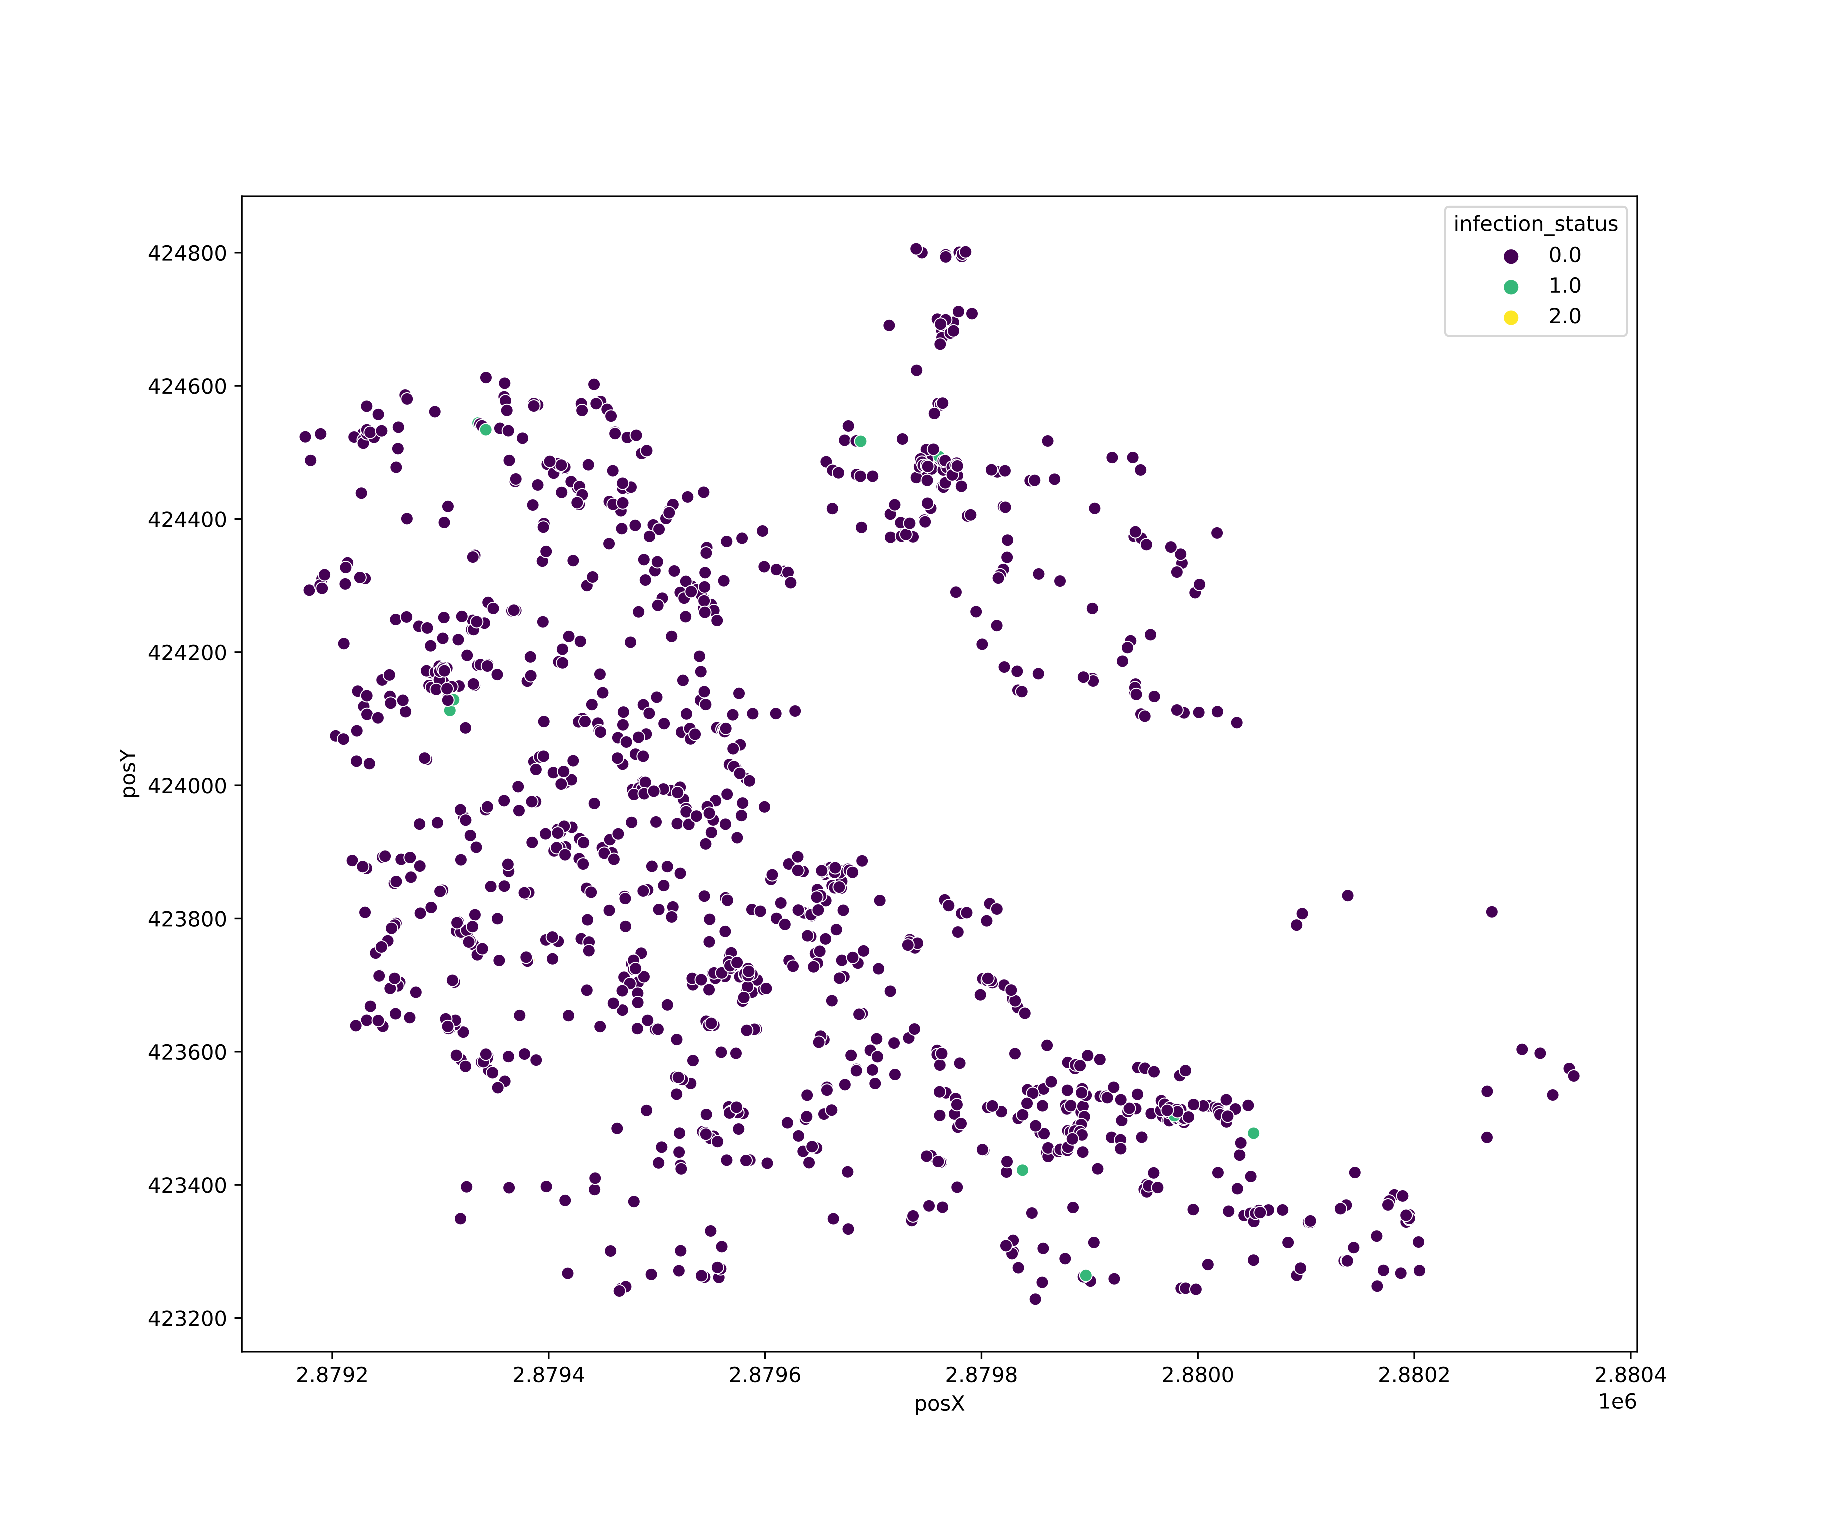
\includegraphics[scale=.5]{fig2}
%\caption{\label{fig} Spatially Explicit Spread on the Miami Citrus B2 Dataset. The area of the B2 survey was approximately $15.5km^2$, and there are approximately 1100 hosts (citrus trees) present. \cite{Gottwald2002}} 
%\end{figure} 

The population size is $N$ and is constant. Hosts may move between the following compartments: $S$, $C$, $I$ and $R$.

\begin{equation}
	S(t) + C(t) + I(t) + R(t) = N(t) = N,   \forall t \ge 0 
\end{equation}

At time $t = 0$, $C_0$ hosts are randomly infected. The $C_{0}$ hosts are cryptic: they do not show symptoms but may transmit infection to other hosts. A preexisting control programme involves surveys of the host population at a frequency every $\Delta$ days, and a symptomatically infected host of type $i$ is detected with probability $p_i$. The time of the first control event, $\Delta_{0}$ days, is randomly selected from the  $[0, \Delta]$ interval, to reflect an ongoing 'preventative control' programme aimed at preventing the incursion of invasive plant disease, and the unpredictability of when an incursion of pathogenic material may occur. If the host is cryptically infected the infection is detected with probability 0, and with $p_{d, i}$ for host of type $i$ in compartment I (symptomatic infected hosts), and this is species-specific. The number of each type detected during a round of control is drawn from a binomial distribution.

If detected, the host is removed, along with any host within a radius of $r_{i}$ m. of the removed host, for a host of species $i$. Often, the radius is the same for both species, $r_{A} = r_{B} = r$.
The single-species model with single-radius control corresponds exactly to the case of constant-radius control examined in \cite{HyattTwynam2017}, where there is a single parameter $r$ which may be optimised for disease control.

To model the propensity for \emph{Xylella fastidiosa} to infect multiple host species or cultivars, the single-host type model was extended to a multi-type model with two host types, denoted as A and B respectively. In the single-type case, transmission is parameterised directly by only one parameter, $\beta$. However, since the pathogen can infect two host types, there is an increased set of parameters in the two-species case. In particular, the transmission of infectious propagules from species A $\rightarrow$ B may occur with a different propensity than B $\rightarrow$ A, or A $\rightarrow $A, in the most general case. This is the asymmetric transmission considered in this work. One way to parameterise the asymmetric transmission is as in \cite{NdeffoMbah2010}, where the transmission matrix is 

\begin{equation}
\label{ndeffo}
\bf{T_{mat}} = 
\begin{pmatrix}
\beta_{AA} & \beta_{AB} \\
\beta_{BA} & \beta_{BB}
\end{pmatrix} 
\end{equation}

with $\beta_{ij}$ the transmission parameter from species $i \rightarrow j$. This constitutes a phenomenological approach, but for the below model, we adopt a slightly different parameterisation which is more biologically inspired but not mathematically distinct from Eq. (\ref{ndeffo}). (It depends on the assumption that all propagules behave the same, irrespective of the host species releasing them.) 

The constant parameterising transmission from individuals of species $i$ to $j$, $\beta_{ij}$, is a product of both the infectivity of the $i$ species ($\nu_{i}$, the susceptibility to infection of the $j$ species $\phi_{j}$, and the permissivity of the environment to the infectious agent $\eta$. Hence, we write

\begin{equation}
\beta_{ij} = \nu_{i} \phi_{j} \eta
\end{equation}

and for $j \rightarrow i$:

\begin{equation}
\beta_{ji}= \nu_{j} \phi_{i} \eta
\end{equation}



\begin{equation}
    \begin{pmatrix}
\beta_{AA} & \beta_{AB} \\
\beta_{BA} & \beta_{BB}
 
\end{pmatrix} = 
\begin{pmatrix}
\nu_{A} \phi_{A} \eta & \nu_{A} \phi_{B} \eta \\
\nu_{B} \phi_{A} \eta & \nu_{B} \phi_{B} \eta \\
\end{pmatrix}
\end{equation}

$\eta$ reflects the fraction of infectious propagules that - having been released by a primary host - go on to physically reach a potential secondary host. $\eta$ is a function of environmental conditions, but we assume it is equal for all scenarios here and thus remove it: 

\begin{equation}
\label{nuphi}
   \bf{T_{mat}} = 
\begin{pmatrix}
\nu_{A} \phi_{A} & \nu_{A} \phi_{B} \\
\nu_{B} \phi_{A} & \nu_{B} \phi_{B} \\
\end{pmatrix}
\end{equation}

We also incorporate species-specific crypticity, since different species are likely to manifest symptoms at different times after infection (relevant to $\sigma$) and potentially to different extents (relevant to probability of detection, $p_d$). Hence the nature of crypticity for the two host-type system is summarised in the following matrix

\begin{equation}
   \bf{S_{mat}} = 
\begin{pmatrix}
\sigma_{A} & \sigma_{B} \\
p_{d,A} & p_{d,B}\\
\end{pmatrix}
\end{equation}

The stochastic dynamics in the absence of control are governed by the following equations where $\Psi$ denotes the transition rate of an individual:

%\end{eqnarray}array}
\label{twospecies}
    
%\end{equation}
\begin{eqnarray}    
\Psi \left( S_{A} \rightarrow C_{A}\right) &=& \phi_{A} \left( \nu_{A} \sum_{i \in C_{A}(t), I_{A}(t)}^{} K(d_{ij}; \alpha) + \nu_{B} \sum_{i \in C_{B}(t), I _{B}(t)}^{} K(d_{ij}; \alpha) \right) \\
   \Psi \left( C_{A} \rightarrow I_{A}\right)  &=&  \sigma_{A} \\
   \Psi \left(I_{A} \rightarrow R _{A}\right) &=& \gamma \\
%\label{twospeciesB}
    \Psi \left( S_{B} \rightarrow C_{B}\right) &=& \phi_{B} \left( \nu_{A} \sum_{i \in C_{A}(t), I_{A}(t)}^{} K(d_{ij}; \alpha) + \nu_{B} \sum_{i \in C_{B}(t), I _{B}(t)}^{} K(d_{ij}; \alpha) \right) \\
   \Psi \left( C_{B} \rightarrow I_{B}\right) &=&  \sigma_{B} \\
  \Psi \left(I_{B} \rightarrow R_{B}\right) &=& \gamma 
\end{eqnarray}



\begin{figure}[h]
	\centering
	\includesvg[scale=1.8]{compartment}
	\vspace*{5mm}
	\caption{ \label{compartmentdiag} \textbf{Compartmental diagram of the multitype SCIR model in the absence of control events.} $S_i$ (green fill): Susceptible hosts of type $i$. Both $C_i$ (cryptically infected hosts, yellow fill) may transmit infection to susceptibles of either type with infectivity $\nu_{i}$. Susceptibles of type $i$ are vulnerable to infection with susceptibility $\phi_{i}$. The progression rate of $C_{i}$ to $I_{i}$ (symptomatic infecteds, red fill) is governed by the type-specific rate parameter $\sigma_{i}$. Following symptom development, hosts die at a rate $\gamma$ equal for both types. Dead hosts are in the removed compartment ($R_{i}$, grey fill) and are permanently inactive.}
	\end{figure}


For the spatial stochastic model, the two potential kernel functions $K(d_{ij}; \alpha)$ considered are the thick-tailed Cauchy kernel and the thin-tailed exponential kernel, which have the forms given in \cite{HyattTwynam2017}. Both of these functions are parameterised by the dispersal scale $\alpha$, although the Cauchy kernel gives a higher probability of long-distance dispersal events than the exponential kernel.
The system is simulated stochastically using Gillespie's Direct Simulation Algorithm \cite{Gillespie1977} as outlined in \cite{Keeling2008} with the following detail: when a time-step would move the epidemic time to later than a scheduled control event, the the control event was performed and time re-set to the control time, before recalculating transition times for each host and an associated time-step. The main simulation was performed in a parallelised manner using the custom Python 3 script  $\texttt{gillespie\_dsa.py}$.

\FloatBarrier
\subsection*{Model parameterisation from \emph{Xylella} studies}

The model formulated here is not, and does not aim to be, predictive. However, efforts have been made to place parameter values within biotic ranges so that the qualitative dynamics of the control problem can be examined. 

\subsubsection*{Crypticity Parameters: $\sigma$ and  $p_{d}$}

  EFSA provide several species-specific estimates for $\sigma_{i}$ in \cite{Bragard2019}. Specifically, the estimated mean asymptomatic time is $\frac{1}{452}$ days$^{-1}$ for \emph{Olea europea} infected by \emph{X. fastidiosa subsp. pauca}. However, the estimated median asymptomatic time for this pathosystem via parametric and non-parametric methods respectively given in \cite{Bragard2019} lead to estimates of $\frac{1}{203}$ and $\frac{1}{452}$ days$^{-1}$ for the asymptomatic period. An additional complexity is that the SCIR model assumes that hosts are instantaneously infectious to others following infection, but this is not realistic \cite{Leclerc2014}. Instead, there is a non-zero incubation time, not explicitly modelled here. In view of the considerable uncertainty on precise quantification and in addition the simplistic nature of exponentially distributed residence time in the Cryptic compartment, $\sigma$ is set to either $\frac{1}{350}$  days$^{-1}$ (less cryptic) or $\frac{1}{500} \mathrm{days^{-1}}$ (more cryptic).
\FloatBarrier
\subsubsection*{Dispersal Kernel and Scale Parameter of \emph{Xylella fastidiosa}}

In \cite{White2017}, a grid-based approach (in contrast to the present model) was used to model and predict the early spread of \emph{X. fastidiosa} in Apulia, Italy. Dispersal in that case was argued to be stratified, with long-distance dispersal events occurring. Hence, two separate dispersal mechanisms were incorporated, an exponential kernel to model shorter dispersal events, parameterised by $\alpha = 100 m$, and a longer-range dispersal generator (2D Gaussian). A simpler approach taken here is the use of the thicker-tailed Cauchy dispersal kernel, in combination with the thinner-tailed exponential kernel which is $K_{\exp}(d; \alpha) = \exp\left(\frac{-d}{\alpha}\right)$ as in \cite{HyattTwynam2017}. 

\emph{Xylella fastidiosa} is primarily vectored in the European Union (EU) by the spittlebug \emph{Philaenus spumarius} \cite{Bragard2019}\cite{Bodino2021}. Mark-release-recapture (MRR) provides quantification of the dispersal rate of the vectors through time. MRR was used in \cite{Bodino2021} to estimate a Gaussian dispersal kernel at different times following vector release. 50\% of spittlebugs stayed within 200m over the course of 6 months in an olive grove setting in Apulia, Italy. Using the cumulative distribution function formula (CDF) for a 2D normalised exponential dispersal kernel, this median value implied a scale parameter of 119 m for the exponential kernel. Since the Cauchy kernel $K(d_{ij}; \alpha) = \frac{1}{1+\left(\frac{d_{ij}} {\alpha}\right)^2}$ cannot be normalised in $\mathbb{R}^2$, the scale parameter for this kernel was derived via least-squares fitting using script $\texttt{fit\_ls.R}$ to the exponential kernel ($\alpha_{\mathrm{expon.}}=119$m), giving a scale parameter for the Cauchy kernel of $\alpha_{\mathrm{cauchy}}= 84.5$m.
In the short range eco-epidemiological model \cite{Bragard2019}, susceptibility of the host plant was defined by as the average probability a host is systemically infected following 1 day of feeding by an infected vector. Hence, asymmetric transmission was implemented as type A having lower susceptibility than type B. In symmetric cases, the value of $\phi_{i}$ set equal in both host types. 
\FloatBarrier
\subsection*{Normalisation and Epidemic Termination Condition}

To compensate for the differences in kernel forms and host densities, normalisation was conducted for each landscape-parameter combination, such that $\mathbb{E(K_E, t = 500 d. = \frac{N}{2}}$ for a population of N hosts.
The simulation termination condition is: $S(t) = 0$ or $C(t) + I(t) = 0$. Epidemic impact, $K_{E}$ is computed as 

\begin{equation}
    K_{E} = C(t) + I(t) + R(t)
\end{equation}

once $C(t) + I(t) = 0 $ or $ S(t) = 0$. 

\begin{table}
\centering
\begin{adjustbox}{width=\textwidth}
\small
    \begin{tabular}{|c|c|c|c|c|}
    \thickhline
         \textbf{Host Type Identity (if appl.)}  & \textbf{Parameter Description} & \textbf{Parameter Symbol} & \textbf{Values} & \textbf{Source}\\
         \thickhline
        \thickhline
         \emph{O. europea} infec. \emph{X.f. subsp. pauca} & Symptom appearance rate & $\sigma_{A}$& $\frac{1}{350}$ day$^{-1}$ &  \cite{Bragard2019}\\
         \thickhline
                  \emph{O. europea} infec. \emph{X.f. subsp. pauca} & Symptom appearance rate & $\sigma_{B}$& $\frac{1}{350}$ or $\frac{1}{350}$ day$^{-1}$ &  \cite{Bragard2019}; see text\\
        \thickhline
         \emph{O. europea} & Death rate (I) & $\gamma$  & 0.00053 day$^{-1}$&  \cite{Bragard2019} \\
        \thickhline
        Generic & Susceptibility to infection& $\phi$& 0.09 or 0.14 & \cite{HyattTwynam2017}\\
        \thickhline
        Generic & Infectivity & $\nu$ & fit via normalisation & N/A \\
        \thickhline
        \emph{X. fastidiosa subsp. pauca}& Exponential Kernel Scale Parameter & $\alpha_{\mathrm{exp}}$ & 119 m & Median fit to \cite{Bodino2021}\\
        \thickhline
        \emph{X. fastidiosa subsp. pauca}& Cauchy Kernel Scale Parameter & $\alpha_{\mathrm{cauchy}}$ & 84.5 m & Least-squares fit to $\alpha_{\mathrm{exp}}$ \\
        \thickhline
    \end{tabular}
    \end{adjustbox}
    \caption{Parameter values and sources used for this study: Host Demography and Infection Processes. See text for details of fitting performed.}
    \label{demography}
\end{table}


\begin{table}
    \centering
    \begin{adjustbox}{width=\textwidth}
    \begin{tabular}{|c|c|c|c|c|}
    \thickhline
        \textbf{Species Identity}  & \textbf{Parameter Description} & \textbf{Parameter Symbol} & \textbf{Values} & \textbf{Source} \\
        \thickhline \thickhline
        e.g., Olive & $\mathbb{P} \mathrm{(detected\:|\:surveyed\:type\:A)}$& $p_{d,A}$& 1 & \cite{Bragard2019} \\   
        \thickhline
         Cryptic Host & $\mathbb{P} \mathrm{(detected\:|\:surveyed\:type\:B)}$& $p_{d,B}$& 0.2 & None\\        
        \thickhline
         N/A & First survey time & $\Delta_{0}$& Rand*[0,90] & None\\
        \thickhline
        N/A & Survey interval & $\Delta$ & 90 days&  \cite{HyattTwynam2017}\\
        \thickhline
         Olive-like & Fraction surveyed (A)  & $F_{A}$ & 1 &  \cite{HyattTwynam2017}\\
        \thickhline
         Cryptic host & Fraction surveyed (B) & $F_{B}$ & 1 & \cite{HyattTwynam2017}\\
        \thickhline
    \end{tabular}

    \label{controlparms}
        \end{adjustbox}
    \caption{Control-related parameters used for this study. }
\end{table}

\FloatBarrier
\subsection*{Landscape Generation and Parameter Sweeps}

In all cases, the total number of hosts in the model, $N$, was set at 1110 to upper bound computation time, and approximately follow previous work \cite{HyattTwynam2017}. For each parameterisation, 5 landscape instances were generated, with 50 epidemics performed on each instance giving 250 replicates for each generative landscape parameterisation.


\begin{table}

    \begin{tabular}{|c|c|c|c|}
    \thickhline
        \textbf{Landscape Model} & Number of hosts & Landscape Area & \textbf{Density}
     \\
        \thickhline \thickhline
        CSR: Low Density Regime & 1110 & 16km$^{2}$ & 69.4 hosts/km$^{-2}$ \\
        \thickhline
        CSR: Medium Density Regime & 1110 & 9km$^{2}$& 123.3 hosts/km$^{-2}$ \\
        \thickhline
        NS: Low Density Regime & 1110 & 16km$^{2}$ &  69.4 hosts/km$^{-2}$ \ \\
        \thickhline
            \end{tabular}
    \caption{   \label{lscapes} Landscapes used in this study}
\end{table}

For each landscape considered, the radius of host removal was varied on an interval of [0,1200] m to find the approximate optimal radius of removal with respect to Median ${K_{E}}$. Additional epidemic outcome metrics were Area Under the Disease Progress Curve (AUDPC) (modified from \cite{Cunniffe2015}) and the epidemic impact per host type. Results for each landscape were written out as summary statistics to csv files by the script \texttt{pd\_fig.py}.
 Computation of an approximately optimal control strategy occurred by simply selecting the radius of removal which gave the lowest median $K_E$ or the lowest median AUDPC depending on the subplot. This was graphically compared to the 'misspecified control' strategy which was defined to be the optimal radius (with respect to, 'w.r.t.', $K_E$) when landscape was composed solely of type A hosts.

%Survival analysis was conducted by computing the time for which each host was infectious (if at all), separated by host type where appropriate. Then, if multiple replicates of the epidemic were plotted together, the survival function was divided by the number of hosts infected to give a function mapping to [0, 1]. The mean fraction of type $i$ hosts, $S_{i}(t)$, still infectious at $t$ days post-infection was computed across 250 replicates except where otherwise noted. All survival analysis was performed using the custom script \texttt{survival.py}. 


\begin{figure}[h]
	\centering
	\includesvg[scale=0.4]{epidemics}
	%\includesvg[scale=0.5]{olive.svg}
	%%\includegraphics[scale=0.5]{Rplot01.eps}
	\caption{ \label{epi_nocontrol} \textbf{Progression of an uncontrolled epidemic on a host landscape of complete spatial randomness.} Half of hosts are type B and approximately half the total hosts are infected by 500d (as expected under normalisation condition. Host deaths begin to be significant towards $T = 750$ days. Parameterisation is $\emph{Xylella}$-like (see Methods). Host density $\approx 123$ hosts km$^{-2}$, and $N = 1110$. }
\end{figure}
\FloatBarrier
\section*{Results}
	\subsection*{Epidemic Metrics and Theoretical Foundations} 
	Brief formulation of governing equations was performed. In particular, Area Under Disease Progres Curve (AUDPC) as previously defined \cite{Cunniffe2015} was no longer suitable for asymmetric cases and a type-corrected AUDPC was computed in all simulations.
	Export of infectious material to areas outside the modelled square domain is a significant risk, and if the surrounding area has economic or cultural value similar to the comparatively small domain modelled, then success of control of invasive disease then also depends on the export of infectious materials during the course of the epidemic inside the modelled area. AUDPC gives some measure of this potential for export \cite{Cunniffe2015} of infectious material in an epidemic ending at time $\tau_{e}$: 
	\begin{equation}
	\mathrm{AUDPC} = \int_{t = 0}^{\tau_{e}}\left( C(t) + I(t)\right)  dt  
	\end{equation}
	However, in a multi-type epidemic the infectivity of each host type, $\nu_{i}$, may differ. Hence, calculation of the modified AUDPC 
	\begin{equation}
		\mathrm{AUDPC} = \int_{t = 0}^{\tau_{e}} \left( \sum_{i} \nu_{i} (I_{i}(t) + C_{i}(t)) \right) dt
	\end{equation}

	 I also remark that, modifying \cite{vandenBosch2024} slightly and noting Eq. \ref{nuphi} gives:
	
	\begin{equation}
		R_{0, i} = \nu_{i} \Bigl(\frac{1}{\sigma_{i}} +  \frac{1} {\gamma} \Bigr)   \int_{0}^{\infty} \Bigl(  2 \pi r D(r) \left( O_i(r)\phi_{i} + O_{j}(r)\phi_{j} \right) \Bigr) dr
	\end{equation}
	for the basic reproductive number of a type $i$ host. The pathogen has dispersal kernel $D(r)$ and susceptible host type $i$ occur with density $O_{i}(r)$ at distance $r$ from the infected host.  Then for a radius of control $\mathrm{rad}_{\mathrm{removal}}$:
	
	\begin{equation}
		\label{gnocont}
		R_{\mathrm{escaped}, 0} = \nu_{i} \Bigl(\frac{1}{\sigma_{i}} +  \frac{1} {\gamma} \Bigr) \int_{\mathrm{rad}_\mathrm{removal}}^{L}  \Biggl( 2 \pi r D(r)\Bigl( O_i(r)\phi_{i} + O_{j}(r)\phi_{j} \Bigr)\Biggr) dr
	\end{equation}
	
	where $R_{\mathrm{escaped},0}$ gives the number of secondary infections established outside the host removal zone if the primary infected host were to be detected immediately. 
	
	Eq. \ref{gnocont} provides an explanatory framework for the dynamics of epidemics at early time, but does not incorporate periodic surveying and radial removal processes.  Nevertheless, it provides testable predictions for the effect of landscapes on the epidemic. 
	
%	A survival function $S(t)$ can also be computed, giving the fraction of hosts ever infected during the epidemic still infectious to others, at time $t$ after being infected. In the absence of control, 
	
%	We have
%	$0 \ge S(t) \le 1, \forall t > 0$. 
	
%	For a host of type $i$ write $S_{i}(t)$, so that the survival functions may be compared across types. The area under the survival curve conforms to 
	
%	\begin{equation}
%		\int_{t=0}^{t_{end}} S_{i} dt = \frac{AUDPC(i)}{N_{i} \nu_i}
%	\end{equation}



%In \textbf{Fig. \ref{epi_nocontrol}} the uncontrolled epidemic parameterised for \emph{Xylella} qualitatively exhibits approximately wave-like fronts expanding from the multiple initial sites of infection. The epidemic ends due to host death since control is not applied, as can be seen from the later panels. 


\FloatBarrier
%\subsection*{Effect of Crypticity Parameters on Control in the Single-Type Case}


%For a thick-tailed Cauchy kernel, simply varying $p_d$ on [0, 1] with control optimised perturbs mean epidemic impact as follows: 

%%\begin{figure} [hbt!]
%\includegraphics[scale=.4]{pd.eps}
%\includegraphics[scale=1]{detection_sweep.eps}
%\caption{\label{fig} Misspecification of detection probability causes approximately linear decay in control efficacy for the Cauchy kernel as quantified by $K_E$. Parameters as in \cite{HyattTwynam2017}. }
%\end{figure}

%This approximately linear increase in epidemic impact, $K_{E}$, corresponds to a misspecification of the detection probability parameter. This is plausible. Hence, the efficacy of constant radius of removal control does not exhibit abrupt nonlinearities if $p_{d}$ is incorrectly assumed to be 1, at least for the parameters and kernels chosen. This is as expected from the governing equations for the system \ref{}.  

%\begin{figure}
%\includesvg[scale=0.8]{2d_draft_sweep.svg}
%\caption{\label{fig} Radial control performs differently across different probabilities of detection, in the Citrus Landscape. Optimal radius of removal is landscape dependent.}
%\end{figure}

%Other parameters may also be misspecified. Specifically, $\sigma$, which parameterises residence time in the Cryptic %compartment, may be misspecified. Assuming control is optimised for the nominal value of $\sigma =  $, then the% expected final size varies as in 

%\includegraphics[scale=1]{sigma_sweep.eps}


\subsection*{Q1: How does increasing proportion of host type B influence control?}

In general, an increase in both epidemic impact ($K_E$) and area under the disease progress curve (AUDPC) was observed as the fraction of cryptic host (type B) was increased. This trend persisted even if the control was optimised to the landscape considered. 

\textbf{Fig \ref{1d}} shows a 1-dimensional parameter sweep with a clear optimal radius of removal w.r.t. $K_E$ at approximately 400m. At a low radius of removal ($r_\mathrm{rem}$ < 300m), the majority of hosts are infected. However, if  the radius of removal is too large, then an approximately linear increase in $K_E$ is observed since excessive removal of susceptible hosts occurs. This makes sense in view of the homogeneous density of hosts and expected number of hosts within a circle of radius. However, since presence of a more cryptic host type in the landscape often changes the optimal radius of control,  this method was repeated with cryptic hosts present at increasing proportion to give \textbf{Fig \ref{csr4kdeltapd}}.

\begin{figure}[h]
	\centering
	\includesvg[scale=0.4]{1dscan.svg}
	\vspace{10mm}
	\caption { \label{1d} \textbf{Median epidemic impact $K_{E}$ shows a clear optimum under varying radius of control.} Median $K_E$ (brown dot) is shown with quartiles 10-30 of $K_E$ (Q10-Q30) and Q70-Q90 (both light blue fill) of the $K_E$ distribution, and Q30-Q70 is shown in darker blue fill. A relatively sharply defined optimal radius of removal is at approximately 400m. Host density of 69.3 hosts /km$^{-2}$ on a square landscape of type A hosts only, with 1110 total hosts. Parameterisation is for \emph{Xylella} with $\sigma_{A}$ = $\frac{1}{350}$ days$^{-1}$, with an exponential dispersal kernel. 1000 epidemics performed per point at 50 m step-size, with 200 replicates for each of 5 landscapes.}
	\vspace{10mm}
\end{figure}


\begin{figure}[h]
	\centering
	\includesvg[scale=0.6]{csr_4k_deltapd_exp}
	\caption{\label{csr4kdeltapd} \textbf{The effect of increasing the proportion of host type B, with $p_{d,B}  = 0.2$}. $\sigma_{A} = \sigma_{B} = \frac{1}{350}  \mathrm{days}^{-1}$. Epidemic metrics were computed for host landscapes of complete spatial randomness with $\approx 70 \: \mathrm{ hosts} / \mathrm{km}^2$. \textbf{A)} The optimal radius of host removal generally increases as the proportion of cryptic hosts rises when measuring the Median epidemic impact $K_E$. \textbf{B)} The same epidemics as for A), but AUDPC computed as the dependent variable. Near-Optimal AUDPC is attainable for a far broader range of control radii than optimal $K_E$.  
		Optimal radii show a less pronounced trend with a smaller impact on Median AUDPC. Each block is 250 replicates at a resolution of 50 m.}
\end{figure}

For a landscape with $\approx$ 70 hosts/km$^{2}$ (the low-density case) and distributed homogeneously according to complete spatial randomness (CSR), the $K_E$ showed a clear optimum (\textbf{Fig \ref{csr4kdeltapd}A}) at $r_{\mathrm{removal}} \approx$ 400m when only type A hosts were present. Under this control radius, approximately 550 hosts of 1110 were lost to removal or disease ($K_E = 550$). As the fraction of host type B increased, the optimal radius exhibited a clear increase to a maximum of $\approx 750$ m, although for the landscapes composed mostly of host type B (frac(B) = 0.8, 1.0) the control had begun to fail, as the significant majority of hosts ($K_E > 800$) were lost. Hence, increasing proportion of host type B damaged the radial control programme even under landscape-specific control radius optimisation to minimise $K_E$.  The AUDPC (\textbf{Fig \ref{csr4kdeltapd}B}) showed a weaker trend with a putative small increase in optimal radius from ~ 950m at frac(B) = 0 to $\approx$ 1150m at frac(B) = 1. The distributions of $K_E$ were more sharply-peaked than those of the AUDPC as response variable. This reflects the cost associated with increasing removal radius as more uninfected hosts are removed. By contrast, in the AUDPC case, a more aggressive control strategy with larger radius is rewarded, as there is no penalisation of excess host removals and instead absolute minimisation of the infection pressure applied by the modelled patch is desired. The AUDPC was increased approximately 5-fold from maximal removal radius (1200m) and frac(B) = 0 to frac(B) = 1 and $r_\mathrm{removal} = 0m$. This would indicate an approximately 5-fold greater risk of disease export to the 16 km$^{2}$ patch surroundings. There is significant divergence between the optimal strategies if radius is optimised for $K_E$. \textbf{Fig. \ref{deltacompare4kcsr}} illustrates this by solely comparing optimal control for each degree of host type heterogeneity with optimal control for frac(B) = 0. The misspecified control strategy (i.e., removal radius 400m in this case) led to approximately twice the median AUDPC than for the lanscape optimised case. However, the median $K_E$ exhibited closer correspondence between the landscape adapted case and the type A misspecified control case than median AUDPC response variable did.


\begin{figure}
	\centering
%\includesvg[scale=.85]{4k_exp_csr_deltapd_misspecified.svg}
\includesvg[scale=0.75]{delta_compare_exp_csr_4k}
\caption{\label{deltacompare4kcsr} \textbf{Differential degradation of control efficacy as frac(B) $\rightarrow 1$ depending on control strategy.} Both landscape-optimised (with respect to $K_{E}$ in \textbf{A} and AUDPC \textbf(B)) and misspecified controls degrade in effectiveness as the proportion of cryptic ($p_{d,B} = 0.2$) hosts rises. \textbf{(A)} shows the close similarity in control efficacy, as measured by $K_E$, as the fraction of host type B increases. \textbf{(B)}: The increase in AUDPC is more pronounced for the misspecified control case, and exhibits significant divergence away from landscape-adapted control as shown by the lack of overlap in interquartile ranges for frac(B) $>$ 0.5. Epidemic data from Fig \ref{csr4kdeltapd}. [A small X-jitter has been applied to prevent bar overlap.]}
\end{figure}
\FloatBarrier
 %For CSR landscape models, varying both removal radius and fraction(B) showed an increase in optimal radius with increasing landscape crypticity (\textbf{Fig. \ref{csr4kdeltapd}}). 
  \subsubsection*{Thicker-tailed kernels reduce efficacy of radial control and increase export risk under type-heterogeneous landscapes}
 
 The findings above were qualitatively robust to the form of the dispersal kernel. For the thick-tailed Cauchy kernel there was an increased $K_E$ relative to the exponential kernel), indicating that disease was harder to control with an increased probability of dispersal events falling outside a given  control radius. As the fraction of type B hosts increased, the optimal radius of removal with respect to $K_E$ also increased at a significant, constant, rate to a maximum at frac(B) = 1 (\textbf{ Fig. {\ref{cauchy4kdeltapdcsr}}}). Furthermore, comparison of landscape-optimised strategies with the naively misspecified control strategy (that is, optimal radius to minimise $K_E$ with frac(B) = 0), then no overlap between the two strategies was observed (textbf{Fig. \ref{cauchydivergence}B). Importantly \textbf{Fig. \ref{cauchydivergence}} shows that an adaptive radius of control on an increasingly type-heterogeneous landscape does not perform significantly better than the misspecified strategy, if $K_E$ is the response variable of interest. 
 
 \begin{figure}
 	\centering
 	\includesvg[scale=0.40]{cauchy_final.svg}
 	\caption{\label{cauchy4kdeltapdcsr} \textbf{The Cauchy kernel reduces control efficacy but optimal radius of removal still increases with frac(B) $\rightarrow 1$.} \textbf{A)} Median epidemic impact ($K_{E}$) in the Cauchy kernel case is very high: approximately 900 of total 1110 hosts are infected or removed at optimum, even when all hosts are type A. Hence, control essentially fails in this case, for the given survey interval $\Delta = 90$ days. \textbf{(B)} shows that long radii of removal ($>1 $km) are favoured to reduce AUDPC to optimal values for nearly all landscapes considered.
 		 Host density 69.3 hosts/km$^{-2}$, and a CSR host distribution.}
 \end{figure}
 
 \begin{figure}
 	\centering
 	\includesvg[scale=0.40]{cauchydivergence4000.svg}
 	\caption{\label{cauchydivergence} \textbf{The thick-tailed Cauchy kernel exhibits marked divergence in AUDPC when misspecified control is used, compared to optimal control for the CSR landscape considered.} Finite-patch effects are at play: the graph (\textbf{(A)} Increasing landscape heterogeneity does not increase $K_E$ ) .  Note the upper-bounding of $K_E$ at high frac(B) since nearly all hosts are infected in either control radius strategy. \textbf{(B)} The AUDPC for control minimising $K_E$ is divergent from control minimising AUDPC, even without presence of two host types. Significant difference between the two distributions in AUDPC remains at increasing frac(B).}
 \end{figure}
  
 \FloatBarrier
 \subsection*{Q2: Two Forms of Crypticity: Is the $\Delta \sigma$ Case Different to $\Delta p_{d}$?}

  
 Both longer cryptic periods ($\Delta \sigma$) and reduced probability of infection detection once symptomatic ($\Delta p_{d}$) are plausible mechanisms for increased crypticity in an alternate host. Hence, the case where $\sigma_{B} < \sigma_{A}$ was examined (\textbf{Fig \ref{sigma4kcsrsym}}). The general increase in optimal radius of removal (w.r.t. $K_E$) as $\mathrm{frac(B)} \rightarrow 1$ was robust to whether the crypticity was a reduced probability of detection or a longer cryptic period.
However, with $\sigma_{B} = \frac{1}{500} \mathrm{days}^{-1}$ and $ p_{d,B} = 1$ there was a more modest and constant rate increase in the optimal radius with respect to $K_E$ (\textbf{Fig. \ref{sigma4kcsrsym}}) than for the previously treated $\Delta p_{d}$ case, which exhibited a more nonlinear increase in optimal radius of removal. At frac(B) = 1, the optimal radius produced a median $K_E \approx 680$, but a large range of radii (350 - 700 m) gave similar $K_E$. This indicates a lack of system sensitivity to the radius of removal in that regime. 

\textbf{Fig. \ref{compare_strategies_delta_sigma} A} shows an approximately linear increase in $K_E$ under increasing landscape heterogeneity (frac(B) $\rightarrow 1$). There is extensive variance in the $K_E$ distributions. In addition, there is no clear constraint of the results by susceptible host exhaustion, as was noted for the Cauchy kernel case (Fig. \ref{cauchydivergence}). By contrast, \textbf{Fig. \ref{compare_strategies_delta_sigma} B} exhibits a clear divergence between the AUDPC computed for the optimal radii (wrt AUDPC) and the misspecified radius, which did not account for the landscape heterogeneity. Although both responses are approximately linear, the gradient of increase in AUDPC ($\frac{\Delta AUDPC}{\Delta \mathrm{frac(B)}}$) is far greater in the optimised control regime. Furthermore, the variance exhibited in distribution of AUDPC is smaller in the optimised control regime compared to the misspecified radius case, indicating tighter system control. 

\begin{figure}
	\centering
\includesvg[scale=0.6]{sigma_4000_csr_sym.svg}
\caption{\label{sigma4kcsrsym} \textbf{ $\Delta \sigma$ : Optimal radii tend to increase with the fraction of host B  when $\sigma_B < \sigma_A$ and \textbf{$p_{d,A} = p_{d,B}$} = 1}. \textbf{(A)} Optimal radius with respect to $K_E$  shows a less pronounced increase as Frac(B) $\rightarrow$ 1 than for the $\Delta p_{d}$  case (Fig. \ref{csr4kdeltapd}), increasing slightly from 350 m to 500 m. as frac(B) $\rightarrow$ 1. \textbf{(B)} optimal radius of removal with respect to AUDPC shows no clear trend and a flat response for most higher radii ($r_{\mathrm{rem}} > 500m$). Host density $\approx$ 70 hosts km$^{-2}$ and homogeneously distributed (CSR).}
\end{figure}

\begin{figure}[h]
	\centering
\includesvg[scale=0.65]{delta_sigma_4k_csr.svg}
\caption{\label{compare_strategies_delta_sigma} \textbf{Performance of optimal and misspecified control radii for the  case where $\sigma_{B} = \frac{1}{500} \mathrm{days}^{-1}$. (A)} Close correspondence between the misspecified and optimal control strategies persists even as $\mathrm{Frac(B)} \rightarrow 1$ when measuring $K_{E}$.  \textbf{(B)} With AUDPC as the response variable, there is significant divergence between the two strategies, even for the mostly homogeneous landscapes, with $\mathrm{Frac(B)}$ small. $N = 1110$.}
\end{figure}

%Analysis of the time taken for hosts of each type to be removed also reveals longer half-lives (time taken for half the hosts to be removed) in the more cryptic hosts no matter the form which crypticity takes. \textbf{Fig. \ref{halflivesfracB2radius400}} shows that the near-optimal radius of removals compensates for the differential crypticity effect through removals of host type B when host A is detected, since the density of hosts is sufficiently high. This is further evidenced by \ref{} which shows a strong difference in survival 

%\begin{figure}
%	\caption{ \label{halflivesfracB2radius400} \textbf{Survival analysis for the with radius of removal 400m.} There is only a modest difference in half-life of the two host types for a small fraction of type B hosts.}
%\end{figure}


%\begin{figure}
%\includesvg[scale=0.9]{prop_B_JAN.svg}
%\caption{\label{fig5} Emergent nonlinearity in decaying efficacy of control as proportion of Cryptic species increases. The dispersal kernel is Citrus canker-like. Landscape of complete spatial randomness: $16 \mathrm{ km}^2$, 1200 hosts. $p_{d}  = 0.2$ for cryptic species (B) and $p_d$ = 1 for species A. Fixed radius of removal, 31 m. Cauchy kernel, $\alpha = 36.1$m}
%\end{figure}


%\subsection*{Disease Controllability for Equal Mean Detection Probability Diverges Depending on Population Heterogeneity}


%The decay of control efficacy as the mean ${p_d}$ ($\bar{p_{d}}$) of an individual in the population decreases divergent, depending on whether all members of the population have the same $p_d$  or if there is a subset of the population with crypticity ($p_{d} <1$, and all other individuals have $p_d = 1$. Specifically, mean $p_d$ is given by

%\begin{equation}
%\bar{p_{d}} = \frac{n_{A} p_{d,A}  + n_{B} p_{d,B}}{n_{a} + n_{b}} 
%\end{equation}

%with $n_{a} + n_{b} = N$. 

%%
%% need more evidence here, ie one or two graphs
%%



%\begin{figure}
%%\includesvg[]{feb2_sweep_cauchy.svg}
%%\caption{\label{fig7} 
%Optimal radius of removal (chosen from [0,1]km) increases as the proportion of cryptic hosts increases.  
%Landscape of complete spatial randomness: 16km $^2$, 1110 Hosts, with Cauchy Dispersal Kernel ($\alpha = 84.5m$). Optimal radius %highlighted by green circle for each landscape.}
%\end{figure}


 
 

% \subsection*{Q4: Two-Radius Control Shows Modest Benefits}




%If the radius of removal is allowed to be species-specific, $r_{A} \neq r_{B}$, then the potential benefit of this approach can be quantified. 

%For the landscape with frac(B) = 0.5:

% insert figure for Tworadius control here
%\begin{figure}[ht!]
%\includesvg[scale=0.15]{two_radii.svg}
%\caption{ \label{tworadiii} Two-radius control shows only a modest improvement on single-radius control for this parameterisation when measuring $K_E$.}
%\end{figure}

% and maybe have a second case 

\newpage
\FloatBarrier
\subsection*{Q3: Clustering: Control on Neymann-Scott Landscapes}

The Neyman-Scott model allows the clustering of hosts \cite{vandenBosch2024}. The analysis of the clustered landscape is rendered more difficult by the multiple factors which change as frac(B) varies. 

A parameter scan with host types A and B having the same epidemiological parameters showed the impact of landscape patterning on disease controllability is shown in \textbf{Fig. \ref{identicaltypes}}. The more type-heterogeneous landscapes $\frac{N_{B}}{N_{A} + N_{B}} \approx 0.5$ exhibit significantly lower $K_E$ than  more type-homogeneous landscapes.  The increased number of clusters in the heterogeneous landscapes allowed more host sparing and a lower peak local density of hosts. In addition, the optimal removal radii with respect to $K_E$ shown in \textbf{Fig.  \ref{identicaltypes}A} reflect the generative landscape model. The scale parameter for the cluster generation process was 100m, and optimal radius of removal was also 100m. The AUDPC (\textbf{Fig.  \ref{identicaltypes}B)} also showed a reduction for frac(B)  = 0.4,0.6 if the radius was low ($r _{\mathrm{rem}} \approx$ 50m, 100m).


\begin{figure}[h]
	\centering
\includesvg[scale=0.5]{identical_types.svg}
\caption{ \label{identicaltypes} \textbf{Effect of clustering when host A and B are identical.} A higher number of landscape clusters increases disease controllability with a thin-tailed kernel. There is a strongly conserved optimal radius of removal (100m) with respect to $K_E$ \textbf{(A)} but not with respect to the AUDPC, where the radius accounts for less of the variation in values. \textbf{(B)} shows a weak trend in optimal radius of removal w.r.t. AUDPC, whereby lower radii are a suitable control strategy for intermediate frac(B)}
\end{figure}

\begin{figure}[h] % this is the compare controls plot for the 
	\centering
\includesvg[scale=0.5]{compare_equiv.svg}
\caption{ \label{compareidenticaltypes} \textbf{Strong effect of the number of host clusters present on differential performance of optimal and misspecified controls w.r.t AUDPC. (A)} There is a clear optimal fraction of type B hosts for $K_E$, but since optimal radius of control is the same despite type heterogeneity, there is little difference in control strategy w.r.t. $K_E$. \textbf{(B)} By contrast, the choice of control radius is consequential in the case of AUDPC.}
\end{figure}

For the case where host B is more cryptic and the landscape is clustered, there are two cases as before. When $p_{d, B} < p_{d,A} = 1$ then the observed pattern of optimal controls is modulated rather subtly (\textbf{Fig. \ref{pdclust4000exp}}), at least for this landscape parameterisation. This indicates that the effect of  the number of clusters dominates, with the effect of crypticity exerting a moderate perturbation to this. 

\begin{figure}[h]
\includesvg[scale=0.65]{deltapd_clust_4000.svg}
\caption { \label{pdclust4000exp} \textbf{
When host type B has a reduced $p_d$ ($p_{d, B} = 0.2$), the optimal control radius is increased to 150m compared to the less cryptic case.}}
\end{figure}



\begin{figure}[h]
\includesvg[scale=0.55]{clustered_deltapd.svg}
\caption { \label{clustdeltapdcompare} 
\textbf{Divergence between the optimal and misspecified controls for the }
} 

\end{figure}


\begin{figure}[h]
\includesvg[scale=0.76]{delta_sigma_clust}
\caption { \label{sigmaclust4000exp} 
}
\end{figure}

\begin{figure}[h]
\includesvg[scale=0.85]{delta_sigma.svg}
\caption { \label{sigmaclustcompare} $K_E$ \textbf{(A)} panel and AUDPC \textbf{(B)} panel are consistent across optimal and misspecified controls, but exhibit greater divergence in AUDPC \textbf{(B)}.} 
\end{figure}


%\begin{figure}[h]
%\includesvg[scale=0.6]{clustered_deltapdsigma.svg}

%\caption{ \label{deltasigmapd} For the case where $p_{d,B} =0.2$ and $\sigma_{B} = \frac{1}{500}$ days$^{-1}$, these two forms of crypticity interact to produce  } 
%\end{figure}


%\begin{figure}[h]
%\includesvg[scale=0.65]{compare_deltasigmapd.svg}

%\caption{ \label{comparedeltasigmapd}  } 
%\end{figure}

However, the effect of the landscape patterning in

% should illustrate the point about landscapes
%%% perhaps we can compare, or simply have a few landscapes here.
\FloatBarrier
\subsection*{Q4: Asymmetric Transmission: Effect on Control}

Since biotic parameters between types of host may differ, parameter scans under asymmetric transmission were conducted. Specifically, the worse-case scenario from a disease control perspective, where themore cryptic host type B was either more susceptible or infectious to other hosts, was considered. 

In the first case, the more cryptic host (B) was set to be less susceptible than the type A host to the pathogen. Specifically, for a parameter matrix with form  

\begin{equation}
	\begin{pmatrix}
		\nu_{A} & \phi_{A} \\
		\nu_{B} & \phi_{B}  \\
	\end{pmatrix} 
\newline
= \frac{1}{100}
	\begin{pmatrix}
	2 & 0.9 \\
	2 & 1.4 \\
\end{pmatrix} 
\end{equation}

such that 


\begin{equation}
	\begin{pmatrix}
		\beta_{AA} & \beta_{AB} \\
		\beta_{BA} & \beta_{BB} \\
	\end{pmatrix} = 
\eta	\begin{pmatrix}
		\nu_{A} \phi_{A}  & \nu_{A} \phi_{B}  \\
		\nu_{B} \phi_{A} & \nu_{B} \phi_{B} \\
	\end{pmatrix} \\
 = \frac{1}{100^2} \begin{pmatrix}
 1.8  & 2.8 \\
 1.8 & 2.8 \\
 \end{pmatrix} 
\end{equation}

and $p_{d,A} = p_{d,B} = 1$ but $\sigma_{A} = \frac{1}{350} \mathrm{and } \sigma_{B} = \frac{1}{500} \mathrm{days^{-1}}$. 


This modulated the expected epidemic impact and AUDPC in a major way \textbf{Fig. \ref{asym4000}} , causing a sharp increase in optimal radius and also exacerbating divergence between AUDPC in the misspecified and optimal control cases even at low frac(B) \textbf{Fig. \ref{asym4000compare}}




% which transmission matrix used here?? 
% 
%

\begin{figure}[h]
	\centering
\includesvg[scale=0.3]{asym_4000.svg}
\caption{ \label{asym4000} \textbf{Asymmetric transmission: type B set as more susceptible than type A. } The optimal radius increases far more sharply than in previous cases.}

\end{figure}


\begin{figure}[h]
	\centering
\includesvg[scale=0.4]{asym_4000_compare.svg}
\caption{ \label{asym4000compare} For asymmetric transmission, the two control strategies show extreme divergence with respect to AUDPC, indicating that asymmetric transmission exacerbates the risk of invasive disease when the more cryptic host type is also more susceptible. }

\end{figure}


% insert results here
% perhaps also the graphical kernel??? 


%\subsection*{Sensitivity Analyses and Alternate Parameterisations}

%\subsubsection*{Survey Interval, $\Delta$}
%The survey interval $\Delta = 90$ days was treated as a fixed variable for this study. However, more frequent surveying could lead to an increase in disease controllability, via two mechanisms: i) hosts with low $p_d$ have more trials to be succesfully detected and initiate a removal event, and ii) hosts emerging from C $\rightarrow$ I could be detected sooner. Hence, simulated epidemics were run for survey interval of $\Delta = 60 \mathrm{ days}$.

%\subsubsection*{Host Number and Landscape Area}

%The number of hosts examined here is comparatively small, and so are the modelled square landscapes.
%However, it is important to consider any potential artefacts of this small N and $L^{2}$, as . 


%Hence, several simulated epidemics were run for N = 10 000, but with the same host density as previously investigated. Small-patch effects affecting the shape of the epidemic progression could include the exhaustion of susceptible hosts for particular parameter ranges, leading to an apparent nonlinearity not directly due to the varying control parameters alone. 
  
\section*{Discussion}

This work has considered some of the complex factors modulating the differential performance of control strategies according to landscape heterogeneity. Only a subset of possible factor combinations have been examined, and there is significant scope for further work. 

The results found above largely agree with existing thinking on crypticity and host heterogeneity. However, the impact of clustering was seen to lower the optimal radius of control both with respect to $K_E$ and AUDPC. This is in contrast to the results found in \cite{Parnell2010} where optimal radius increased with the degree of aggregation in the landscape. This illustrates the potential for divergent control dynamics dependent on the nature of the cluster model, and that further work should required to fit accurate clustered landscape models to host distributions.

\subsection*{Improving Metrics: Limitations of AUDPC as a Proxy for Disease Export Risk}

The AUDPC is an important metric as it summarises the amount of infectious inoculum produced by a patch over the course of an epidemic. However, since the dispersal kernel is montonically decreasing, the infectious pressure exerted by the modelled patch on the surroundings is not necessarily directly proportional to the AUDPC. An epidemic taking place primarily at the boundary of the patch will exert more infectious pressure on the surroundings than an epidemic confined to the centre of e.g., a 16 $\mathrm{km^{2}}$ patch. A better proxy for the export of infectious material might be derived from the positioning of several mock hosts at the border of the modelled domain and computing the infectious pressure received over the course of the simulated epidemic. These detector hosts could then integrate the amount of infectious pressure received over the course of the simulation which would give a more refined measure of epidemic risk. 


\subsection*{Key Findings and Implications for \emph{Xylella fastidiosa} Control Programmes}

The results of this work demonstrate that the ability of \emph{X. fastidiosa susbp. pauca} to infect multiple host species complexifies the optimal control strategy. Control programmes must be aware of the diversity of hosts present within a particular region and to what extent these hosts are susceptible to the circulating strain of \emph{Xylella}. If this is not performed, then a significant increase in AUDPC and outbreak risk in the surrouding area is likely. 

Another key finding was the interaction between asymmetric transmission,  and increased crypticity in the type B host, where AUDPC divergence between misspecified and optimal controls was especially significant. This indicates potential for interacting factors to exacerbate the negative effects of host-type heterogeneity on disease control.

\subsection*{Limitations of the Modelling Approach}

The problem of long-distance dispersal and epidemiology on larger scales has not been addressed. There is some evidence that \emph{Xylella} transport by motor vehicles causes dispersal events at larger scales. To incorporate this, a similar approach to \cite{White2017} could be taken by having two kernels.c Another major limitation of the model is the intra-host dynamics of \emph{Xylella}. Bacterial replication is likely to change infectivity of the tree over time, and in some respects the present analysis is a worst-case scenario since the infectivity of the host is immediate and constant once inside the Cryptic compartment. The clustered landscapes generated here are crude, and a closer parameterisation to real world distributions could also be performed.

\subsection*{Further Work}

Better characterisation of vector biology and behaviour in particular is required, especially for a rigorous predictive modelling study on \emph{Xylella}. Any such predictive study should also incorporate potential effects of climate change on vector distribution \cite{GimenezRomero2024}. Such a model can then guide those developing \emph{Xylella} control programmes through elucidating potential risks to efficacy caused by host heterogeneity.  Further work could also include the development of a metapopulation model incorporating high-density regions of susceptible plants. This may better capture the long-distance transmission which can occur with \emph{Xylella} \cite{White2017}. In parallel with this, the behaviour of growers and policymakers has not been considered in this work (beyond levels of knowledge about the host landscape), even though grower decision-making is known to exert significant influence on disease control \cite{MurrayWatson2022}. Since the results here and in \cite{Cunniffe2015} have shown that more aggressive control strategies (larger radius of removal) are better when minimising AUDPC (but not $K_E$), there is likely to be a conflict between desired nonlocal control (preventing disease export) and the goal of preserving hosts in a grower's patch. This is especially relevant to Olive Quick Decline Syndrome (OQDS) as olive trees affected are sometimes very old and have significant cultural and economic value to growers \cite{Russo2020}. Growers are likely to be reluctant to remove apparently healthy hosts.  For invasive disease, the probability should be on slowing or stopping incursion of the disease into novel areas, and preventing its establishment. Modelling behavioural tension and how to resolve this fundamental conflict is a significant avenue for future work. 
 
 \section*{Supporting information}

\subsection*{Code}

All relevant code, including the primary simulation tool, landscape generators and plotting scripts, are available at ... [TBD] \hyperbaseurl{https://github.com/vargasrichards/IIproj}

All 2D parameter scan data is available in the \texttt{FINALRESULTS} subdirectory. The file \texttt{result\_reader.py} can generate plots based on the report files, as long as the file path is explicitly specified to the script.


% Include only the SI item label in the paragraph heading. Use the \nameref{label} command to cite SI items in the text.

\section*{Acknowledgments}

I thank Prof. Nik Cunniffe for his careful and encouraging supervision, and members of the Cunniffe group for stimulating discussion. 

%
%\clearpage



\printbibliography


\end{document}